%!TEX root = ../proteoform_suite_manual.tex
%---------------------------------------------------------------------
%	CYTOSCAPE VISUALIZATION
%---------------------------------------------------------------------

\section{Visualizing Proteoform Families in Cytoscape}

\subsection{Overview}
Proteoform families are visualized in the software program Cytoscape.\supercite{Shannon2003,Smoot2011} Each node is a proteoform and each edge represents a mass difference between proteoforms, corresponding to a modification or amino acid difference. Proteoform family visualization allows users to visualize all observed proteoforms and modification combinations from each family in a simple graphic. Install Cytoscape version 3.5.0: \url{https://cytoscape.org/download.html}.


\subsection{Visualize Families in Cytoscape}
\begin{itemize}
	\item Export scripts for Cytoscape either on the Proteoform Families page or the Results Summary page
	\begin{itemize}
		\item Cytoscape\_style\_timestamp: file Cytoscape uses to correctly style visualized proteoform families
		\item Cytoscape\_nodes\_timestamp: file containing node information for visualized proteoform families
		\item Cytoscape\_edges\_timestamp: file containing edge information for visualized proteoform families
		\item Cytoscape\_script\_timestamp: script for Cytoscape to load in the style, nodes, and edges file and visualize proteoform families
	\end{itemize}
	\item In Cytoscape, select Tools $>$ Execute Command File.... 
	\item Select the cytoscape\_script\_timestamp file generated by Proteoform Suite
	\item Proteoform families will appear! Should take about 1 min for larger proteoform families.
\end{itemize}
\begin{figure}[h]
\centering
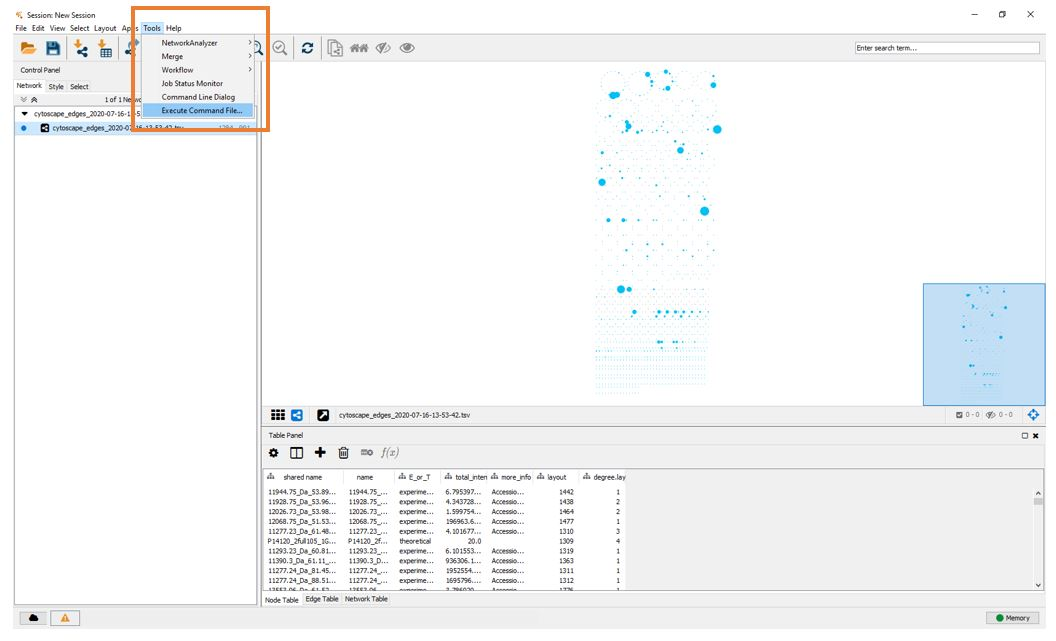
\includegraphics[scale=0.45]{figures/cytoscape1.jpg}
\end{figure}

\pagebreak
\subsection{Proteoform Families Key}
\begin{itemize}
	\item Pink square: gene name
	\item Green nodes: theoretical proteoforms
	\item Blue nodes: experimental proteoforms; size of node is proportional to summed intensity
	\item Purple nodes: top-down proteoforms
	\item Edges: mass differences between proteoforms
	\item Specialized
	\begin{itemize}
		\item Quantified Proteoform families: pie chart for each experimental proteoform shows abundance ratio between two conditions (blue and yellow)
		\item Bottom-up data: orange nodes are bottom-up peptides. Edges indicate that the peptide could be derived from connected the proteoform node
	\end{itemize}
\end{itemize}
\begin{figure}[h]
\centering
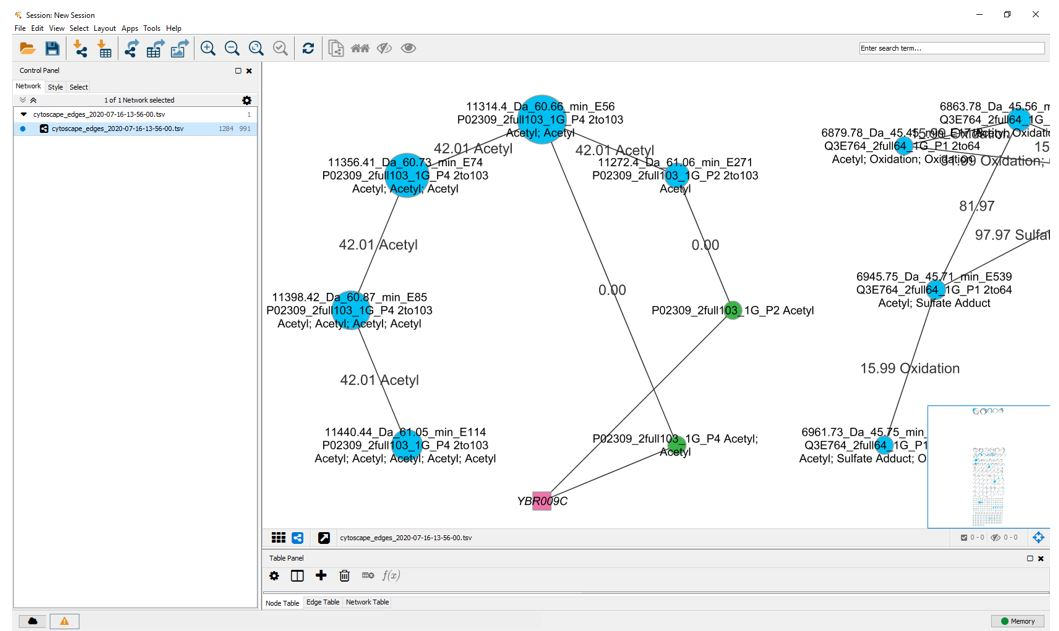
\includegraphics[scale=0.5]{figures/cytoscape2.jpg}
\end{figure}

\subsection{Exporting Family Visualizations into Adobe Illustrator}
\begin{itemize}
	\item In Cytoscape, File $>$ Export $>$ Network View as Graphics...
	\item Select SVG
	\item This will export everything in view into a format that can be loaded by Adobe Illustrator and polished there for publication
\end{itemize}



